\chapter{若当标准形}

本讲我们将在前面讨论的基础上实现复数域上相似标准形理论的终极目标,即得到复数域上全体线性变换都可以得到的一种比较简单的矩阵表示——若当标准形. 我们将讨论其存在与唯一性,并在证明唯一性的过程中给出一种求解若当标准形的方法. 最后,我们将讨论若当标准形的应用.

\section{若当标准形的存在性}
回顾\autoref{thm:15:不变子空间与分块对角矩阵},我们知道寻找线性变换$T\in\mathcal{L}(V)$在基下简单的表示矩阵的一般思路是将$V$分解为一系列不变子空间的直和. 在对角化一节中我们尝试分解为一维不变子空间的直和,但这并不能对所有的线性变换都成立,于是我们进一步在\autoref{thm:16:广义特征性质}中对于任意的线性变换都利用广义特征子空间实现了这一分解,这也直接导出了\autoref{thm:16:分块对角矩阵}中的分块对角形矩阵表示. 然而我们仍无法满足于将这一矩阵表示作为标准形,因为我们还希望分块对角矩阵中每个分块都要足够简单,即有一定的规律且有较多的零元素,所以我们需要对广义特征子空间做进一步的分解,并且取特定形式的基来实现这一目标. 我们首先看如下例子:

\begin{example}
    设$T\in\mathcal{L}(\mathbf{C})^6$满足
    \[T(x_1,x_2,x_3,x_4,x_5,x_6)=(2x_1+x_2,2x_2+x_3,2x_3,2x_4,3x_5+x_6,3x_6),\]
    则我们很容易写出其在$(\mathbf{C})^6$自然基下的矩阵表示为
    \[\left(\begin{array}{ccc:c:cc}
        2 & 1 & 0 & 0 & 0 & 0\\
        0 & 2 & 1 & 0 & 0 & 0\\
        0 & 0 & 2 & 0 & 0 & 0\\
        \hdashline
        0 & 0 & 0 & 2 & 0 & 0\\
        \hdashline
        0 & 0 & 0 & 0 & 3 & 1\\
        0 & 0 & 0 & 0 & 0 & 3\\
        \end{array}\right)\]
\end{example}

通过这一例子我们观察到线性变换的一种分块对角矩阵表示,其中每个分块都十分简单,很适合作为我们实现为复数域上任意线性变换寻找的标准形. 我们称如上例矩阵表示的每个分块的形式的矩阵为\term{若当块}\index{ruodangkuai@若当块 (Jordan block)},更严谨地,域$\mathbf{F}$上的一个$r$级矩阵形如\[\begin{pmatrix}
    \lambda & 1 &        &   \\
      & \lambda & \ddots &   \\
      &   & \ddots & 1 \\
      &   &        & \lambda
\end{pmatrix}\]
则称其为一个$r$级若当块(1级显然就是1阶矩阵),记作$J_r(\lambda)$,其中$\lambda$是对角线上元素. 若一个线性变换$T$在基$B$下的矩阵表示是对角块均为若当块的分块对角矩阵,则称这个分块对角矩阵是线性变换$T$的\term{若当标准形}\index{ruodangxing@若当标准形 (Jordan canonical form)},而这组基$B$称为$T$的\term{若当基}\index{ruodangji@若当基 (Jordan basis)}. 我们希望复数域上任意线性变换都能找到一组若当基使其矩阵表示为若当标准形,而这正是本节需要证明的目标.

为了证明这一结果,我们需要首先观察若当块能在怎样的基下表示出. 为了发现这一规律,我们考虑一种最简单的情况,即一个线性变换$T$在某组基$B=\{v_1,v_2,v_3,\cdots,v_n\}$下的矩阵表示就是一个若当块,即
\[T(v_1,v_2,v_3,\cdots,v_n)=(v_1,v_2,v_3,\cdots,v_n)\begin{pmatrix}
    \lambda & 1 &        &   \\
      & \lambda & \ddots &   \\
      &   & \ddots & 1 \\
      &   &        & \lambda
\end{pmatrix},\]
所以我们根据线性映射矩阵表示的定义可以得到
\begin{align*}
    Tv_1&=\lambda v_1,\\
    Tv_2&=\lambda v_2+v_1,\\
    Tv_3&=\lambda v_3+v_2,\\
    &\cdots\\
    Tv_n&=\lambda v_n+v_{n-1}.
\end{align*}

我们稍作变换,可以得到
\begin{align*}
    (T-\lambda I)v_1&=0,\\
    (T-\lambda I)v_2&=v_1,\\
    (T-\lambda I)v_3&=v_2,\\
    &\cdots\\
    (T-\lambda I)v_n&=v_{n-1}.
\end{align*}

即我们需要的这组基实际上具有如下形式:
\[B=\{(T-\lambda I)^{n-1}v_n,(T-\lambda I)^{n-2}v_n,\cdots,(T-\lambda I)v_n,v_n\},\]
并且有$(T-\lambda I)^n=0$. 事实上观察上面这组等式,从第一个式子我们知道$v_1$实际上是$T$关于特征值$\lambda$的特征向量,$v_2,\cdots,v_n$则是关于特征值$\lambda$的广义特征向量. 这样的一组基在接下的讨论中占有相当重要的地位,因此我们需要写下一个定义描述它:
\begin{definition} \label{def:18:循环基}
    设$T\in\mathcal{L}(V)$,$v\in V$是关于特征值$\lambda\in\mathbf{C}$的一个广义特征向量. 设$n$是使得$(T-\lambda I)^n v=0$成立的最小正整数,则称$\{(T-\lambda I)^{n-1}v,(T-\lambda I)^{n-2}v,\cdots,(T-\lambda I)v,v\}$是$T$关于特征值$\lambda$的一组长度为$n$的循环基,其中$(T-\lambda I)^{n-1}v$称为其起始向量,$v$称为其终止向量.
\end{definition}

给出这一定义后,我们自然地会有以下几个问题:
\begin{enumerate}
    \item 这组向量被称为``循环基'',它真的满足基的基本要求:线性无关吗?
    \item 上面我们只考虑了特殊情况,即线性变换在某组基下矩阵表示为若当块,但我们的目标是证明线性变换有一组基使得其矩阵表示为分块对角矩阵,每一对角块为若当块. 所以循环基长成的子空间是否为不变子空间,因为这样才能保证生成一个对角块?
    \item 是否可以找到一组基是由不同的循环基组成的,从而在这组基下的矩阵表示才是若当标准形?
\end{enumerate}

接下来的几个定理将逐一回答这些问题.
\begin{theorem}
    设$T\in\mathcal{L}(V)$,$B$是$T$关于特征值$\lambda$的一组循环基,则
    \begin{enumerate}
        \item $B$是线性无关的;
        \item $B$生成的子空间$W$是$T$的不变子空间,我们称其为循环子空间.
    \end{enumerate}
\end{theorem}
\begin{proof}
    \begin{enumerate}
        \item
        \item
    \end{enumerate}
\end{proof}

\begin{theorem}
    设$T\in\mathcal{L}(V)$,$\lambda\in\mathbf{C}$是$T$的一个特征值. 设$B_1,\cdots,B_q$都是$T$关于特征值$\lambda$的一组循环基,且它们的起始向量各不相同且构成了一组线性无关向量组,则
    \begin{enumerate}
        \item $B_i(i=1,\cdots,q)$是互不相交的;
        \item $B=B_1\cup\cdots\cup B_q$是线性无关向量组.
    \end{enumerate}
\end{theorem}
\begin{proof}
    \begin{enumerate}
        \item
        \item
    \end{enumerate}
\end{proof}

接下来我们便可以证明本节最核心的一个结果,即关于一个特征值的广义特征子空间有一组由互不相交的循环基并起来构成的基,从而我们可以进一步利用广义特征子空间分解得到每个线性变换都有一组基使得其矩阵表示为若当标准形:
\begin{theorem}
    设$V$是$\mathbf{C}$上的有限维线性空间,$T\in\mathcal{L}(V)$,$G_\lambda$是关于特征值$\lambda$的广义特征子空间,则$G_\lambda$有一组由不相交的关于$\lambda$的循环基取并集构成的基.
\end{theorem}
\begin{proof}

\end{proof}

这一定理还表明同一个特征值对应的广义特征子空间不一定只由一组若当基张成,基并非一个特征值对应一个若当块,这是一个初学时需要注意的误区,下一节讨论若当标准形的求解时读者会了解到若当块的个数是如何决定的.

\begin{corollary} \label{cor:18:若当基存在}
    设$V$是$\mathbf{C}$上的有限维线性空间,$T\in\mathcal{L}(V)$,则存在一组基$B$使得$T$在$B$下的矩阵表示为若当标准形.
\end{corollary}
\begin{proof}

\end{proof}

接下来我们需要描述矩阵的若当标准形. 实际上,线性变换在某组基下有若当标准形与矩阵有相似标准形为若当标准形是等价的. 我们考虑$P^{-1}AP=J$,其中$P$为过渡矩阵,$J$为$A$的若当标准形. 我们可以将$A$视为$\sigma(\alpha)=A\alpha$在自然基下的矩阵,于是$\sigma$在\autoref{cor:18:若当基存在} 给出的基(记为$B$)下的表示矩阵的求解方式就是$\sigma(B)=(B)J$,将$B$组成的矩阵记作$P$,由$\sigma$的定义可知,$\sigma(B)=(B)J$等同于$AP=PJ$,即$P^{-1}AP=J$,故如果我们要求矩阵相似于其若当标准形的过渡矩阵,问题转化为求解若当基然后排列成矩阵即可.
\begin{corollary}

\end{corollary}
\begin{proof}

\end{proof}


至此我们已经证明了若当标准形的存在性,接下来我们将讨论若当标准形的唯一性.

\section{若当标准形的唯一性}
在上一小节的最后,我们将求解若当标准形的目标转化为了求解若当基,我们希望有更加算法化的方式去实现这一目标. 为此,我们先引入一些记号. 我们记$G_j(\lambda,\sigma)=\ker (\sigma-\lambda I)^j$,根据核空间增长以及极小多项式的结论,我们知道当$i<j$时有$G_i(\lambda,\sigma)\subseteq G_j(\lambda,\sigma)$,并且当$\sigma-\lambda I$的次数为极小多项式中该特征值对应因式的次数后,核空间会停止增长.

我们可以优先考虑幂零线性变换$N\in \mathcal{L}(V)$,最后再考虑非幂零的情况应当给我们的算法加什么样的步骤. 我们的目标是求出一组基形如
\[N^{m_1}v_1,\ldots,Nv_1,v_1,\ldots,N^{m_n}v_n,\ldots,Nv_n,v_n,\]
这里有两组未知量,我们依次来说明如何求解. 在求解之前,我们需要引入一个定理表明下述方法的合理性:
\begin{theorem}
    设$\sigma\in \mathcal{L}(V)$,若$V$中向量$v\in G_j(\lambda,\sigma)\backslash G_{j-1}(\lambda,\sigma)$,则
    \begin{enumerate}
        \item 对任意的$i<j$,有$(\sigma-\lambda I)^iv\in G_{j-i}(\lambda,\sigma)\backslash G_{j-i-1}(\lambda,\sigma)$;

        \item $v,(\sigma-\lambda I)v,\ldots,(\sigma-\lambda I)^{j-1}v$线性无关.
    \end{enumerate}
\end{theorem}

\begin{proof}

\end{proof}

这一定理对于下述算法中若当基的阶梯形排列的合理性是必要的,接下来我们开始描述我们的算法. 需要说明的是,这并非求解若当标准形的唯一算法,但这是最契合\autoref{thm:22:若当基存在} 的一种算法,通过这一算法我们能从较为本质的层面求解若当标准形.
\begin{enumerate}
    \item \textbf{\heiti 求解 $\boldsymbol{m_1,\ldots,m_n}$}

          我们首先确定幂次参数,这一参数确定后若当形矩阵就确定了,因为若当形矩阵中每个若当块的大小是$(m_i+1)\times(m_i+1),\enspace i=1,\ldots,n$.
          \begin{enumerate}
              \item 我们假设$m_1\geqslant\cdots\geqslant m_n$,并在接下来的步骤中尝试将若当基重排成如图格式:

                    \begin{figure}[H]
                        \centering
                        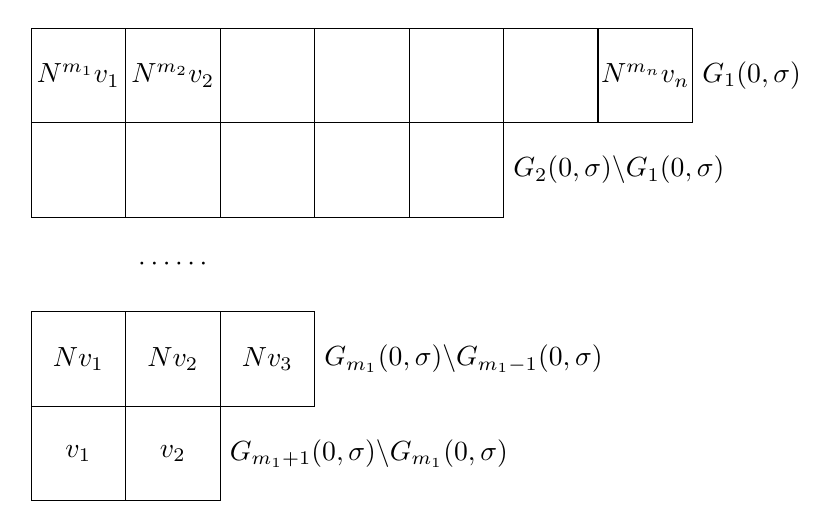
\begin{tikzpicture}
                            \def\F{1.2} % scaling factor

                            \foreach[count=\i] \len in {7, 7, 5, 3, 3, 2}
                                \draw (0, -\F*\i+\F) -- (\F*\len, -\F*\i+\F);

                            \foreach \i in {0,...,2}
                                \draw (\F*\i, -3*\F) -- (\F*\i, -5*\F);
                            \draw (3*\F, -3*\F) -- (3*\F, -4*\F);

                            \foreach \i in {0,...,5}
                                \draw (\F*\i, 0) -- (\F*\i, -2*\F);
                            \foreach \i in {6,...,7}
                                \draw (\F*\i, 0) -- (\F*\i, -1*\F);

                            \foreach \i in {1,...,2} {
                                \node at (\F*\i-.5*\F, -4.5*\F) {$v_{\i}$};
                                \node at (\F*\i-.5*\F, -.5*\F) {$N^{m_{\i}}v_{\i}$};
                            }
                            \foreach \i in {1,...,3}
                                \node at (\F*\i-.5*\F, -3.5*\F) {$Nv_{\i}$};
                            \node at (6.5*\F, -.5*\F) {$N^{m_n}v_n$};
                            \node at (1.5*\F, -2.5*\F) {$\cdots\cdots$};

                            \node[anchor=west] at (7*\F, -.5*\F) {$G_1(0,\sigma)$};
                            \node[anchor=west] at (5*\F, -1.5*\F) {$G_2(0,\sigma) \backslash G_1(0,\sigma)$};
                            \node[anchor=west] at (3*\F, -3.5*\F) {$G_{m_1}(0,\sigma) \backslash G_{m_1-1}(0,\sigma)$};
                            \node[anchor=west] at (2*\F, -4.5*\F) {$G_{m_1+1}(0,\sigma) \backslash G_{m_1}(0,\sigma)$};
                        \end{tikzpicture}
                    \end{figure}

                    即第一行将若当基中在$G_1(0,\sigma)$的向量排列,即在$N$作用一次后就等于0的向量;第二行将所有若当基中在$G_2(0,\sigma)\backslash G_1(0,\sigma)$的向量排列,即在$N$作用一次后不等于0但作用两次等于0的向量,以此类推. 由于假设$m_1\geqslant\cdots\geqslant m_n$,这个图呈阶梯形.

              \item 接下来要将上图填满,首先要确定求解$G_j(0,\sigma)$及其维数(因为幂零线性变换特征值为0)直到$j$等于$N$极小多项式的次数(即幂零指数,或当$G_j(0,\sigma)=V$时),因为此后核空间不可能继续增加,阶梯形也就不会再延伸. 在求出维数后阶梯形状也即确定,因为各层向量个数确定了. 例如假设11维空间中的映射满足$G_1(0,\sigma)$,$G_2(0,\sigma)$,$G_3(0,\sigma)$的维数分别为5,9,11. 这说明从底至上向量个数依次为5,4($=9-5$),2($=11-9$).

              \item 基于上面的求解,这时我们就可以确定若当块的阶数$m_i+1\enspace(i=1,\ldots,n)$,因为这一阶梯中第$i$列的高度实际上就是$m_i+1$(因为每一列是$v_i,Nv_i,\ldots,N^{m_i}v_i$). 将这些若当块拼起来就得到了幂零线性变换的若当标准形.
          \end{enumerate}

          我们将上述讨论总结如下:
          \begin{theorem}
              令$r_j$表示Young图从上至下第$j$行的格数,则有:
              \begin{enumerate}
                \item $r_1=\dim V-r(T-\lambda_i I)$;
                \item $r_j=r(T-\lambda_i I)^{j-1}-r(T-\lambda_i I)^j$.
              \end{enumerate}
          \end{theorem}

          \begin{theorem}
              设$V$是$n$维复向量空间,$T\in \mathcal{L}(V)$,$\lambda_1,\ldots,\lambda_m$为其互异的特征值,则主对角元为$\lambda_j$的若当块的个数$N_j$为
              \[N_j=n-r(T-\lambda_jI)\]
              其中$t$级若当块$J_t(\lambda_j)$的个数$N_j(t)$为
              \[N_j(t)=r(T-\lambda_jI)^{t+1}+r(T-\lambda_jI)^{t-1}-2r(T-\lambda_jI)^t\]
              其中$t$应当小于等于极小多项式中因式$\lambda-\lambda_j$的幂次,$j=1,\ldots,m$. 这个若当形矩阵$A$称为$T$的若当标准形,除去若当块的排列次序外,其若当标准形唯一.
          \end{theorem}
          实际上对于$n$阶矩阵有类似的定理,我们不再赘述. 当我们求解矩阵的若当标准形时,如果我们要求解过渡矩阵,也有简单的方法. 要求$P$使得$P^{-1}AP=J$,则有$AP=PJ$. 假定$P$为$n$阶矩阵,我们可以设$P=(X_1,\ldots,X_n)$,剩下的任务就是解方程了. 因此这种方法非常简单,缺陷在于绕开了若当基这一本质的问题.
          \begin{example}
              利用上述方法求解矩阵\[\begin{pmatrix}
                  2 & 3 & 2 \\ 1 & 8 & 2 \\ -2 & -14 & -3
              \end{pmatrix}\]的若当标准形以及对应的过渡矩阵.
          \end{example}

          \begin{solution}

          \end{solution}

          最后我们需要提到一点,根据上面的叙述,若当标准形在不考虑若当块的排列顺序的情况下是唯一的. 因此任一复数域上矩阵均有唯一的若当标准形(相似标准形),因此我们可以知道,两矩阵相似的一个充要条件是两矩阵有相同的若当标准形(不考虑若当块的排列顺序).

    \item \textbf{\heiti 求解 $\boldsymbol{v_1,\ldots,v_n}$}

          本节内容按照以往的情况在考试中不要求,但为了保证讲义的完整性,我们将求若当基的方法也进行描述.
          \begin{enumerate}
              \item 我们在前述内容中求出了各个$G_j(0,\sigma)$,接下来我们需要利用这些向量将之前确定形状的阶梯内容填满. 我们首先将阶梯最上方的向量确定,实际上就是利用求出的$G_{m_1+1}(0,\sigma)$(也就是$V$)和$G_{m_1}(0,\sigma)$求出二者之差. 似乎很简单,但若仔细思索便会发现线性空间的差并不一定好求. 举一个简单的例子,设$G_{m_1+1}(0,\sigma)=\{\alpha_1,\alpha_2,\alpha_3,\alpha_4\}$,$G_{m_1}(0,\sigma)=\{\beta_1,\beta_2\}$. 这其中出现的所有向量可能都完全不一样,所以作差并不容易. 但我们有一种好方法,如果我们每次从$G_{m_1+1}(0,\sigma)$中挑选两个向量和$G_{m_1}(0,\sigma)$中的两个向量放在一起,如果这四个向量线性无关,这就说明这两个挑出的向量就是作差的结果. 原因在于这相当于$G_{m_1}(0,\sigma)$直和这两个向量长成的空间后得到了$G_{m_1+1}(0,\sigma)$. 如果四个向量线性相关,这说明挑选的向量有在$G_{m_1}(0,\sigma)$中的.

              \item 接下来继续计算第二行中的向量. 实际上算出第一行后第二行中部分向量就已经确定了,例如图上的$Nv_1$和$Nv_2$. 我们这时用类似的方法求解$G_{m_1}(0,\sigma)$和$G_{m_1-1}(0,\sigma)$的差,如图只需要确定一个向量,但这一个向量的确定除了要像(a)中一样每次从$G_{m_1}(0,\sigma)$中选择一个与$G_{m_1-1}(0,\sigma)$的基一起判断线性相关性外,还需要确保这个向量和已经求出的$Nv_1$和$Nv_2$是线性无关的,因为它们构成$G_{m_1}(0,\sigma)$的一组基.

                    总结一下,处于$G_j(0,\sigma)\backslash G_{j-1}(0,\sigma)$对应的行的需要补充的向量$v$应当满足如下三个条件:
                    \begin{enumerate}
                        \item $v\in G_j(0,\sigma)$;

                        \item $v\notin G_{j-1}(0,\sigma)$(通过加入$G_{j-1}(0,\sigma)$)的基保证线性无关判断);

                        \item $v$与同一行中左边已求出的向量线性无关.
                    \end{enumerate}

              \item 最后,我们将所有求出的基按照若当基原先的排列顺序重新组合即可. 如果求矩阵相似于若当标准形的过渡矩阵,则按顺序按列摆放即可.
          \end{enumerate}
\end{enumerate}
需要注意的是,我们求解$G_j(0,\sigma)$时实际上都是要用到矩阵形式进行高斯消元的,所以虽然说是基于线性变换,但过程中基本都是矩阵运算.
\begin{example}
    求矩阵\[\begin{pmatrix}
            2 & 3 & 0  & -1 & 2 & -2 \\ -1 & 0 & 2 & 1 & -1 & -2 \\
            1 & 3 & 2  & 0  & 1 & -4 \\ 5 & 6 & -1 & -2 & 5 & -3 \\
            3 & 3 & -1 & -2 & 3 & -1 \\ 1 & 3 & 2 & 0 & 1 & -4
        \end{pmatrix}\]的若当标准形以及相应的过渡矩阵(提示:这一矩阵是幂零指数为3的幂零矩阵).
\end{example}

\begin{solution}

\end{solution}

对于一般的非幂零线性变换,我们需要首先利用第六章中求解特征多项式$f(\lambda)=|\lambda I-A|$的零点的方法求出所有特征值,然后求出各个不变子空间(这一过程实际上也把将来要求的$G_j(0,\sigma)$进行了求解),然后求各个不变子空间上幂零线性变换$(\sigma-\lambda_j)\vert_{G(\lambda_j,\sigma)}$的若当标准形,即我们在$G(\lambda_j,\sigma)$上执行上面所说的算法,注意最后的若当块对角线上为对应的特征值. 对于矩阵$A$,我们将其视为$\sigma(\alpha)=A\alpha$在自然基下的矩阵,然后利用线性变换的方式即可. 同样地,虽然我们是对线性变换进行描述,但是我们求核空间仍然需要基于矩阵,所以我们需要在求出不变子空间后得到分块对角矩阵,然后对各个块进行$A_i-\lambda_jI$的操作化为幂零矩阵然后进行计算.
\begin{example}
    设$A=\begin{pmatrix}
            2 & 1 & 1 \\ -2 & -1 & -2 \\ 1 & 1 & 2
        \end{pmatrix}$,求$A$的若当标准形$J$和矩阵$P$,使得$P^{-1}AP=J$.
\end{example}

\begin{solution}

\end{solution}

\section{若当标准形的应用}
\subsection{求解不变子空间}
在不变子空间一节中我们提到,我们可以利用若当标准形求解不变子空间,如下面的例子:
\begin{example}
    设$V$为$n$维复向量空间,$\sigma\in \mathcal{L}(V)$,$\sigma$在基$\varepsilon_1,\ldots,\varepsilon_n$下的矩阵是一个若当块,证明:
    \begin{enumerate}
        \item $V$中包含$\varepsilon_1$的不变子空间只有$V$自身;

        \item $V$中任意非零不变子空间都包含$\varepsilon_n$;

        \item $V$不能分解为两个非平凡的不变子空间的直和;

        \item $V$中有且仅有$n+1$个不变子空间,它们分别是
              \[\{0\},\spa(\varepsilon_n),\spa(\varepsilon_{n-1},\varepsilon_n),\ldots,\spa(\varepsilon_1,\ldots,\varepsilon_{n-1},\varepsilon_n)\]
    \end{enumerate}
\end{example}

\begin{solution}
    \begin{enumerate}
        \item

        \item

        \item

        \item
    \end{enumerate}
\end{solution}

因此我们如果能将线性变换在一组基下表示为若当块,我们就可以很快地写出其不变子空间.

\subsection{若当标准形与矩阵分解}
接下来我们讨论若当标准形应用于矩阵分解的情形. 我们首先讨论平方根分解,这一点在之前有提及,但此处我们希望从矩阵的角度讨论这一问题.
\begin{theorem}
    在复数域上,设$a\neq 0$,则$J_n(a)$有平方根.
\end{theorem}
我们可以考虑$J_n(\sqrt{a})^2$与$J_n(a)$的关系来证明这一命题.

\begin{proof}

\end{proof}

注意,这里的$a\neq 0$是必须的,因为我们不难证明如下定理:
\begin{theorem}
    当$n\geqslant 2$时,$J_n(0)$不存在平方根.
\end{theorem}

\begin{proof}

\end{proof}

接下来我们考虑之前已经证明的\autoref{thm:20:幂零平方根} \ref*{item:20:幂零平方根:2},即可逆线性变换一定有平方根,我们现在可以使用若当标准形的方式证明,因为可逆线性变换特征值均不为0,因此每个若当块对角线上都不为0,均有平方根,故而得证.
\begin{example}
    定义$\sigma\in \mathcal{L}(\mathbf{C}^3)$为$\sigma(z_1,z_2,z_3)=(z_2,z_3,0)$. 证明不存在$\tau\in \mathcal{L}(\mathbf{C}^3)$使得$\tau^2=\sigma$.
\end{example}

\begin{solution}

\end{solution}

本题为2020年期末考试最后一题,分值25. 实际上只要想到幂零这一要点是很容易的,但若没有思考到位则很容易走偏而失分. 教材8.17给出了两种常见的幂零线性变换,一种是本题这一类型,另一个是微分线性变换,应当熟练掌握.

除此之外,利用若当标准形,我们还可以有以下分解:
\begin{example}
    已知$A$是复数域上的$n$阶方阵,证明:
    \begin{enumerate}
        \item 存在可对角化的矩阵$B$和幂零矩阵$C$,使得$A=B+C$,且$BC=CB$;

        \item 存在复数域上的对称矩阵$B,C$,使得$A=BC$,并且可以指定$B,C$中任何一个为可逆矩阵.
    \end{enumerate}
\end{example}

\begin{proof}
    \begin{enumerate}
        \item

        \item
    \end{enumerate}
\end{proof}

\subsection{求解微分方程}


\subsection{矩阵求幂与马尔可夫链}
若当标准形的另一个应用在于我们可以利用它计算矩阵的幂,因为若当块的幂的计算是简单的:
\[J_k(a)^n=(aE+J_k(0))^n=a^nE+\mathrm{C}_n^1a^{n-1}J_k(0)+\cdots+\mathrm{C}_n^nJ_k(0)^n\]
同时我们也知道$J_k(0)^k=O$(幂零矩阵),所以利用若当标准形求解矩阵的幂是简单的.
\begin{example}
    设$\sigma\in \mathcal{L}(V)$,$v_1,\ldots,v_n$为$\sigma$的若当基,描述$\sigma^2$在这组基下的矩阵.
\end{example}

\begin{solution}

\end{solution}

\section{实数域上的若当标准形} \label{sec:18:实数域上的若当标准形}

\vspace{2ex}
\centerline{\heiti \Large 内容总结}

\vspace{2ex}
\centerline{\heiti \Large 习题}

\vspace{2ex}
{\kaishu }
\begin{flushright}
    \kaishu

\end{flushright}

\centerline{\heiti A组}
\begin{enumerate}
    \item
\end{enumerate}

\centerline{\heiti B组}
\begin{enumerate}
    \item
\end{enumerate}

\centerline{\heiti C组}
\begin{enumerate}
    \item
\end{enumerate}
